\chapter{数据处理}
\section{晴天阴天判断}
根据历史观测的气象数据判度晴天阴天有多种方法,
其中一种比较简单有效的方法是利用总辐射通量密度(即向下短波辐射通量密度)的观测值与理论值的比作为判据进行判断。
目前,有多种模式可以计算总辐射通量密度在晴天时理论值。
简单的模式只需考虑时间、太阳与地球上观测点的相对位置、太阳常数等,
更加准确的模式还会将大气密度、大气压强等因素考虑进去。
本文使用 PVLIB Python \cite{pvlib-github}提供的模式计算向下短波辐射通量密度在晴天时的理论值,
PVLIB Python 实现了 Ineichen-Perez 晴天模式\cite{Ine02}
以及 Simplified Solis 模式\cite{Ineichen2008758},可以根据需要进行选择。

晴天时的向下短波辐射通量密度的理论值与观测值符合的很好,
在得到晴天总辐射通量密度的理论值之后,对一天内进行积分可以得到一天里的总辐射量的理论值 T,
同样对总辐射通量密度的观测值在一天内积分可得总辐射量的观测值 R,令:
\begin{equation}
\alpha = \frac{R}{T}
\end{equation}
当 \(\alpha > 0.7\) 时认为当天是晴天,当 \(\alpha < 0.3\) 时认为当天是阴天。
由此可以利用历史观测的向下短波辐射通量密度结合理论值进行晴天阴天判断。

\section{时间同步与数据校正}
科大站在采集数据后,按照 30 分钟平均值存储在计算机中,而科学岛站采集数据后按 10 分钟平均存储,
为了便于研究,对科学岛站做 30 分钟平均,统一两地的数据采集频率。
科学岛站在 2015 年的 8、9 月份缺失大量数据,
这期间仪器在进行维护,然而为了和科大站进行比较需要选取它们的公共部分,
最终选取了 2015 年 10 月 21 日至 2016 年 6 月 1 日的数据进行分析。

在分析向下短波辐射即总辐射时发现科大站与科学岛站的数据存在微小的相位差,相差 30 分钟左右,
以 2016 年 5 月 25 日和 26 日两天为例,如图\ref{fig:20160525_DSR_raw}:
\begin{figure}[H]
\centering
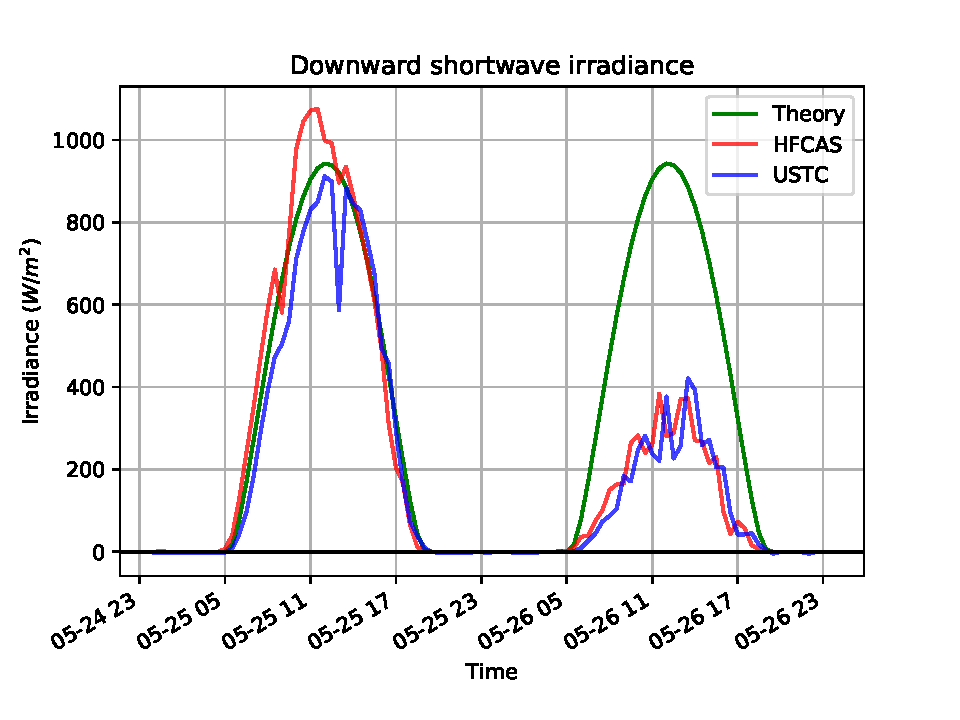
\includegraphics[width=.9\linewidth]{20160525_DSR_raw}
\caption{2016 年 5 月 25 日至 26 日向下短波辐射通量密度原始数据}\label{fig:20160525_DSR_raw}
\note{图中绿色表示向下短波辐射通量密度的理论值,红色表示科学岛站观测的向下短波辐射通量密度, 蓝色表示中科大站观测的向下短波辐射通量密度。 2016 年 5 月 25 日是晴天,2016 年 5 月 26 日是阴天。 从这两天的原始数据中可以看出,与理论值相比,晴天的数据观测值与理论值符合的比较好, 阴雨天由于云层的遮挡,向下短波辐射通量密度会明显降低。 时间上中科大站存在一定的滞后,滞后大约 30 分钟}
\end{figure}
科大站较晚出现向下短波辐射,而两地距离较近,日出时间可以认为相同,且科学岛在科大西边,
因此这个相位差不会是由日出时间差引起,经过分析,这种现象可能是由科大站和科学岛站隶属于不同单位,
两地计算机的时间事先没有很好地同步造成的。
为了对时间进行校正,我们可以先计算出向下短波辐射通量的理论值,在晴天里,
向下短波辐射的理论值与观测值应基本吻合,因此,可以以向下短波辐射的理论值为基准,
对时间作适当修正,即加上或减去一个偏移量,使得两地的时间同步,两地都是在整点或半点采集数据,
发现将科大站的时间轴向左移动 30 分钟后,两地的数据一致性更好,因此取偏移量为 30 分钟。
另外,两地的向下短波辐射通量密度观测值基本都不应超出理论值,
然而科学岛站的原始数据观察发现存在异常偏高,如图\ref{fig:20160525_DSR_raw},
通过对原始数据和向下短波辐射通量密度理论值对比分析,尤其是对晴天数据的认真分析比较,
发现将科学岛的向下短波辐射通量密度乘以 0.86 后与总辐射通量密度的理论值符合的很好,
猜测可能是科学岛站短波辐射测量仪器的灵敏度出现了问题,
相应地向上反射的短波辐射通量密度也乘上了这一修正系数,此后的数据分析研究中使用修正后的数据。
经过时间同步和数据校正之后的结果如图\ref{fig:20160525_DSR},
此时,两地的时间基本同步,向下短波辐射通量密度与理论值符合的也比较好。
\begin{figure}[H]
\centering
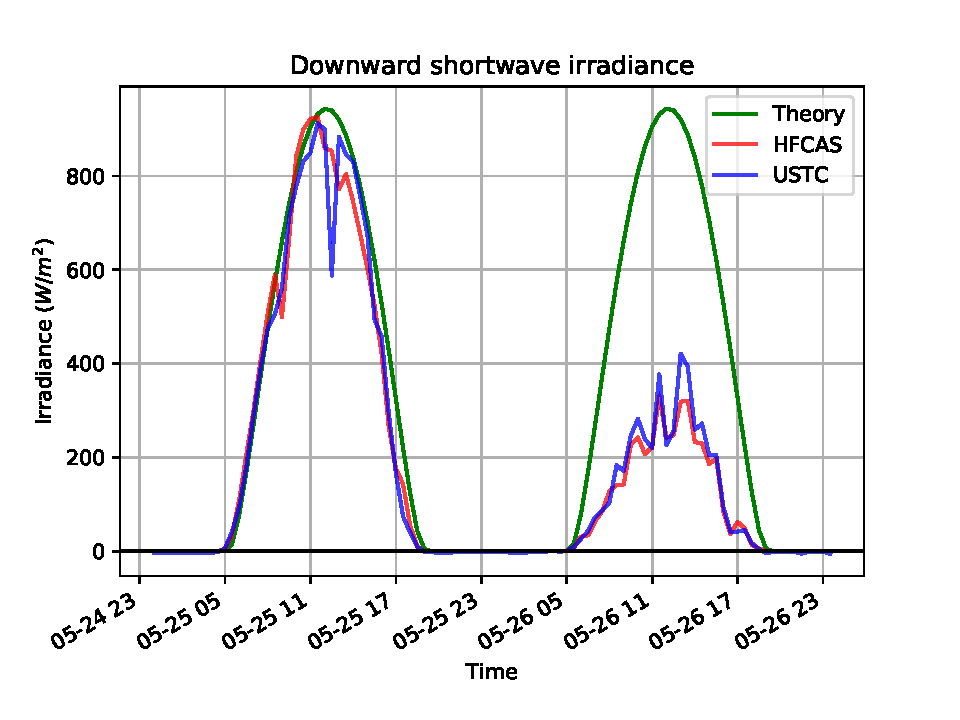
\includegraphics[width=.9\linewidth]{20160525_DSR}
\caption{2016 年 5 月 25 日至 26 日经过时间同步数据校正之后的向下短波辐射通量密度}\label{fig:20160525_DSR}\note{图中绿色表示向下短波辐射通量密度的理论值,红色表示科学岛站观测的向下短波辐射通量密度,蓝色表示中科大站观测的向下短波辐射通量密度。因为数据都是在整点或者半点采集,对科大的原始数据向左移动了 30 分钟,这样既保证了两地时间的同步性,又保证了数据采集时间的一致性。对科学岛的原始数据乘上了 0.86 的修正系数,使得修正之后向下短波辐射通量密度不会高处理论值。}
\end{figure}

\section{野点值去除}
气象观测数据由于受到仪器、天气、环境等各方面因素的影响,通常会存在一些与其它值相差较大的野点。
例如,超声风速仪利用超声发射至反射回来的时间间隔进行测量,
当发生降水过程时,雨滴、冰雪等如果经过超声波的传播路径会对测量结果产生极大干扰。
为了进一步研究分析气象观测数据,需要通过合适的方法将观测数据中的野点值去除。

首先,仪器的观测结果通常用浮点数表示,一些特殊的浮点数如 IEEE 754 中定义的 NaN(not a number)
需要在数据分析前剔除。然后,由于气象数据都是有界的,可以根据历史数据,设定一个经验阈值,
将过高和过低的野点去掉,这种方法虽然简单可行,但经验阈值的设定受主观人为因素影响较大,
我们可以换一种思路:对于大气系统,各气象要素都是连续变化,很少会出现剧烈跳变,
对于某一气象要素时间序列,相邻两个时刻的差值可以认为是一个随机变量,它近似服从正态分布。
由此,为了去除气象要素观测值中的野点,
可先计算该气象要素时间序列后一时刻与前一时刻的差值,即错位做差,
然后通过 3$\sigma$ 原则去除差值大于 3 倍标准差的点。
实际处理数据时,可以先设定一个比较大的阈值区间,将明显没有物理意义的点去除,
然后再通过错位做差 3$\sigma$ 原则去除剩余的野点。
通常这个过程执行一次便可去除绝大多数野点,得到比较理想的结果,如果一次执行后依然存在比较明显的野点,
可迭代多次直到野点全部去除。
潜热通量密度、二氧化碳浓度、水汽浓度等的野点值便通过上述方法去除。

以去除潜热通量密度的野点为例:潜热通量密度的观测受水汽影响较大,出现降水过程会对仪器测量结果产生较大影响,
通过观察原始数据,如图\ref{fig:raw_LE},可以发现中存在较多异常点,只是将图像放大后的结果,
实际的数据中,有些点甚至超过 250000 $W/m^{2}$,这显然是不符合客观事实的,
经过 1 次去除野点的操作之后得到结果如图\ref{fig:LE},
可以看出大部分野点都被除掉。
\begin{figure}[H]
\centering
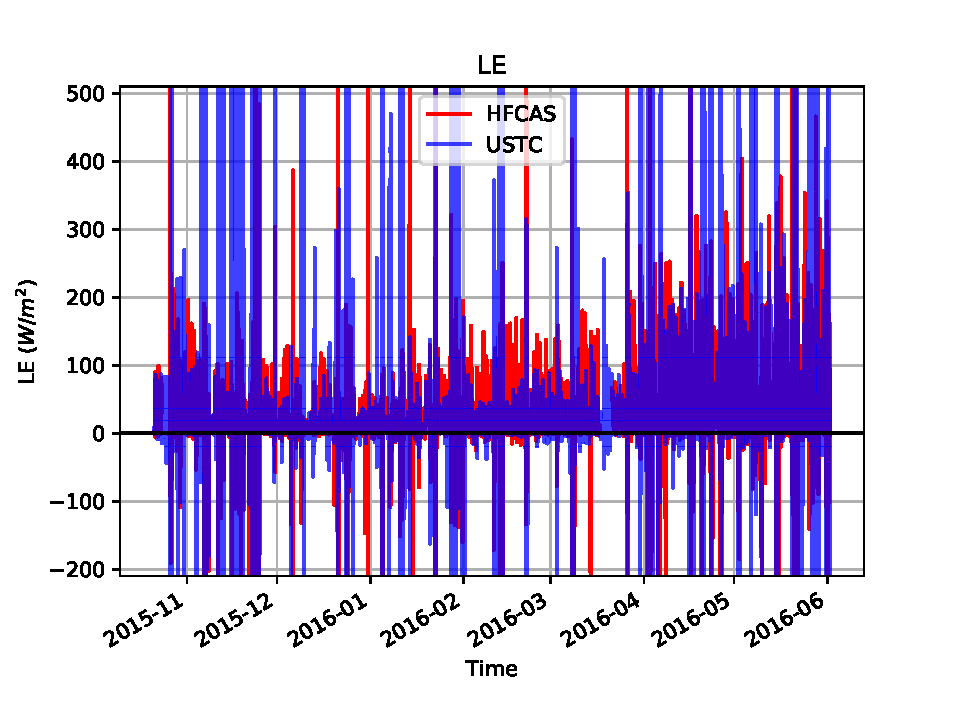
\includegraphics[width=.9\linewidth]{raw_LE}
\caption{潜热通量密度原始数据}\label{fig:raw_LE}
\note{图中红色为科学岛站的潜热通量密度,蓝色为科大站的潜热通量密度。 原始数据中潜热通量密度受到降水的影响存在较多异常点,波动巨大, 而实际的潜热通量密度通常不会超过 400 $W/m^{2}$。}
\end{figure}
\begin{figure}[H]
\centering
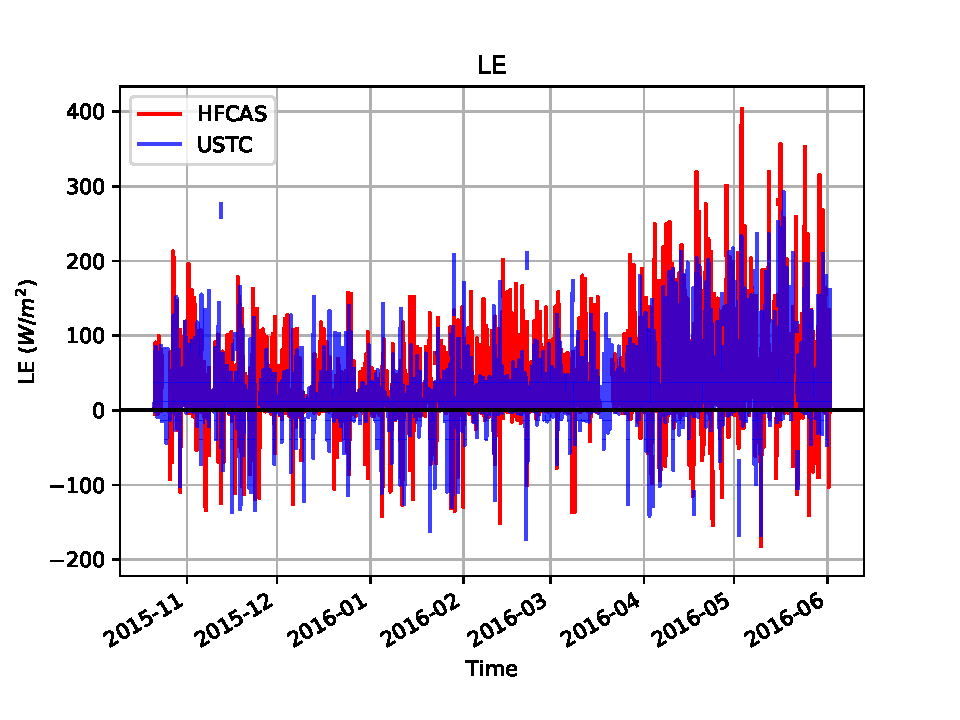
\includegraphics[width=.9\linewidth]{LE}
\caption{去除野点值后的潜热通量密度}\label{fig:LE}
\note{图中红色为科学岛站的潜热通量密度,蓝色为科大站的潜热通量密度。 由于大气运动是一个连续的演化过程,潜热通量密度应具有一定的连续性, 对潜热通量密度的原始数据作错位差,对每一时刻,用下一时刻的值减去本时刻的值, 这一列差值都应维持在一区间内,通过对这列差值的分析,它们近似服从正态分布, 这样便可利用 3$\sigma$ 原则,将绝对值高出 3 倍标准差的潜热数据滤掉。 这是经过一次过滤后的结果,已将大部分野点去除。}
\end{figure}

在处理向上短波辐射时发现,2016 年 1 月 23 日
以及 2016 年 2 月 1 日科大站和科学岛站两地都有出现“异常”偏高,如图\ref{fig:USR}所示。
\begin{figure}[H]
\centering
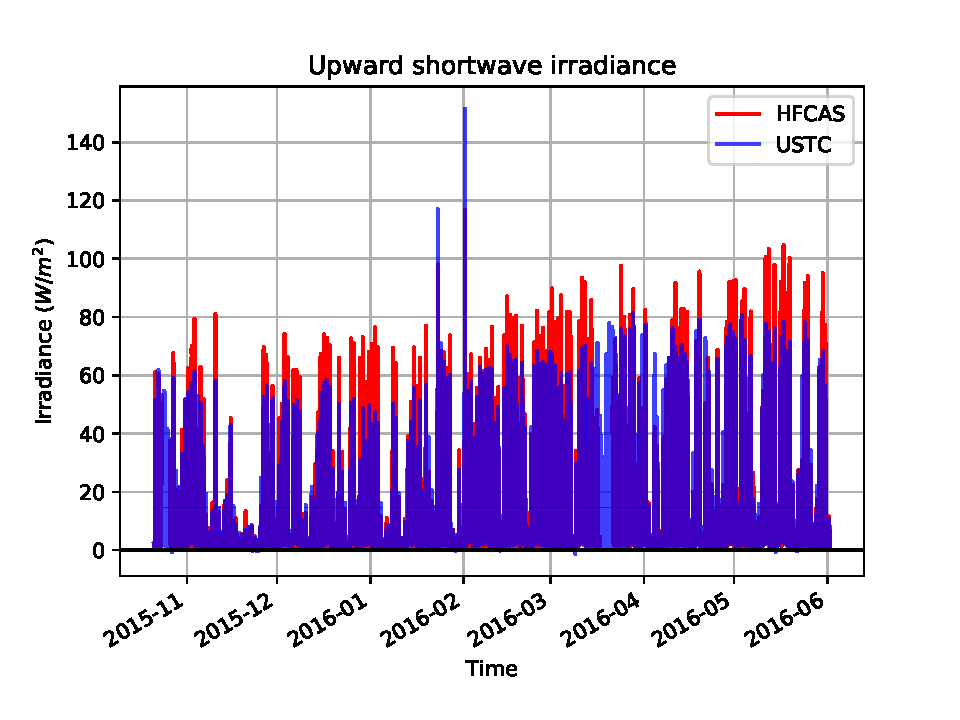
\includegraphics[width=.9\linewidth]{USR}
\caption{向上短波辐射通量密度}\label{fig:USR}
\note{图中红色表示科学岛站的向上短波辐射通量密度,蓝色表示科大站的向上短波辐射通量密度。从图中可以明显看出 2016 年 1 月 23 日以及 2016 年 2 月 1 日向上短波辐射通量密度均出现突增跳变。这种现象可能与降雪有关,积雪导致反照率上升,雪停后向上反射的短波辐射增强。}
\end{figure}
经过进一步研究发现这种向上短波辐射突增的现象与较强的降雪有关:
以 2016 年 2 月 1 日向上短波辐射的突增为例,如图\ref{fig:20160201_USR}:
\begin{figure}[H]
\centering
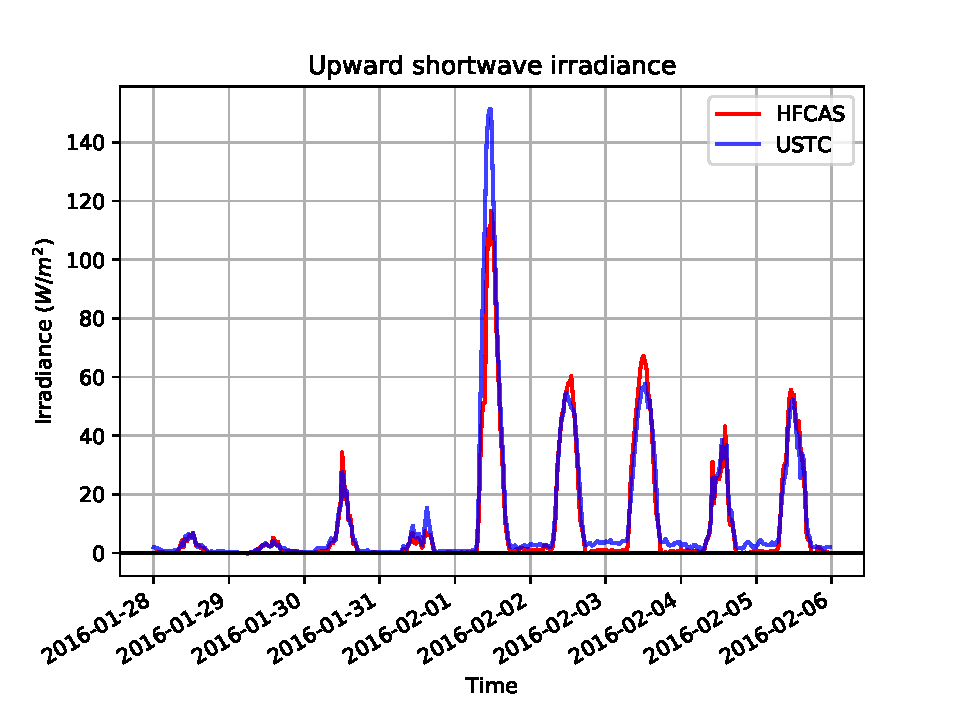
\includegraphics[width=.9\linewidth]{20160201_USR}
\caption{2016 年 1 月 28 日至 2016 年 2 月 6 日向上短波辐射通量密度}\label{fig:20160201_USR}
\note{图中红色表示科学岛站的向上短波辐射通量密度,蓝色表示科大站的向上短波辐射通量密度。 2016 年 1 月 28 日至 1 月 31 日,向上短波辐射通量密度均不超过 40 $W/m^{2}$, 而到了 2 月 1 日中午突增到 100 $W/m^{2}$以上,2 月 2 日以后又降至 60 $W/m^{2}$。}
\end{figure}
从 2016 年 1 月 28 日起至 2016 年 1 月 31 日,向上短波辐射通量密度一直低于 40 $W/m^{2}$,
而到了 2 月 1 日中午,科大和科学岛两地向上短波辐射通量密度均增至 110 $W/m^{2}$ 以上,
2 月 2 日之后又回复到 60 $W/m^{2}$ 附近。
通过图\ref{fig:20160201_DSR}可以看出 2 月 1 日前都是阴天,结合历史天气数据,
2 月 1 日之前发生过一次比较强的降雪过程,2 月 1 日是这次降雪后的第一个晴天。
\begin{figure}[H]
\centering
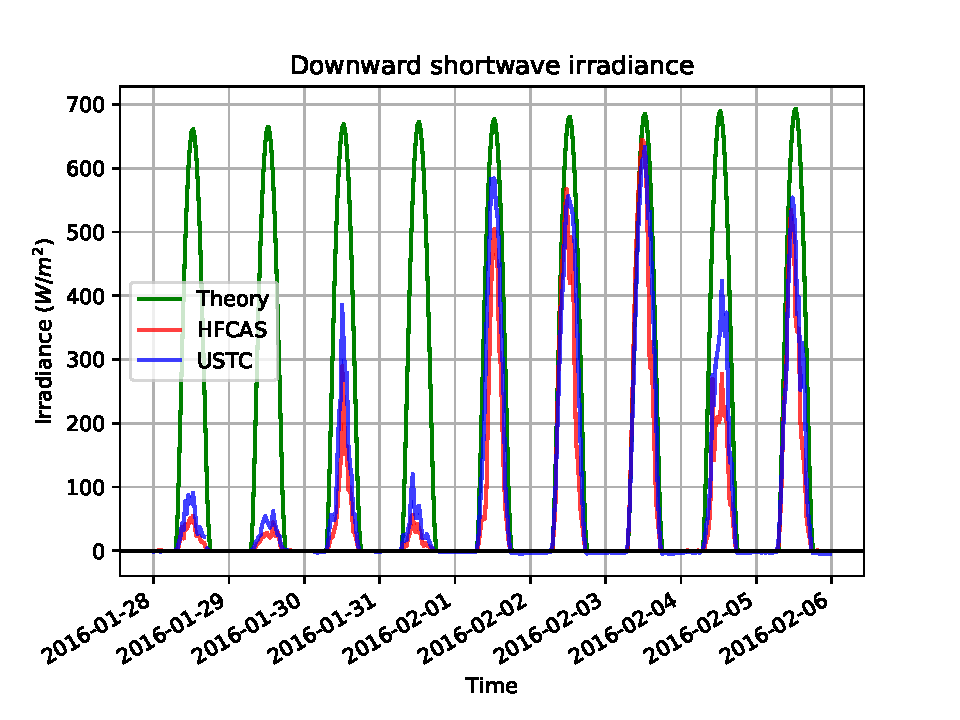
\includegraphics[width=.9\linewidth]{20160201_DSR}
\caption{2016 年 1 月 28 日至 2016 年 2 月 6 日向下短波辐射通量密度}\label{fig:20160201_DSR}
\note{图中绿色表示向下短波辐射通量密度,即总辐射通量密度的理论值, 红色表示科学岛站观测的向下短波辐射通量密度,蓝色表示中科大站观测的向下短波辐射通量密度。 从图中可以看出 2016 年 1 月 28 日起至 2016 年 1 月 31 日均是阴天, 向下短波辐射比较低,同时根据历史气象数据, 1 月 31 日还发生过一次降雪过程。 而到了 2 月 1 日,天气转晴,总辐射升高,晴天一直维持到 2 月 3 日。}
\end{figure}
通过分析 2 月 1 日附近反照率的变化,如图\ref{fig:20160201_albedo}所示,
1 月 31 日中午之前,两地反照率维持在 0.1 附近,1 月 31 日下午反照率突增至 0.6,
2 月 1 日上午两地峰值均超过 0.7,可以推断是这次降雪过程地面积雪增加了地面的反照率。
\begin{figure}[H]
\centering
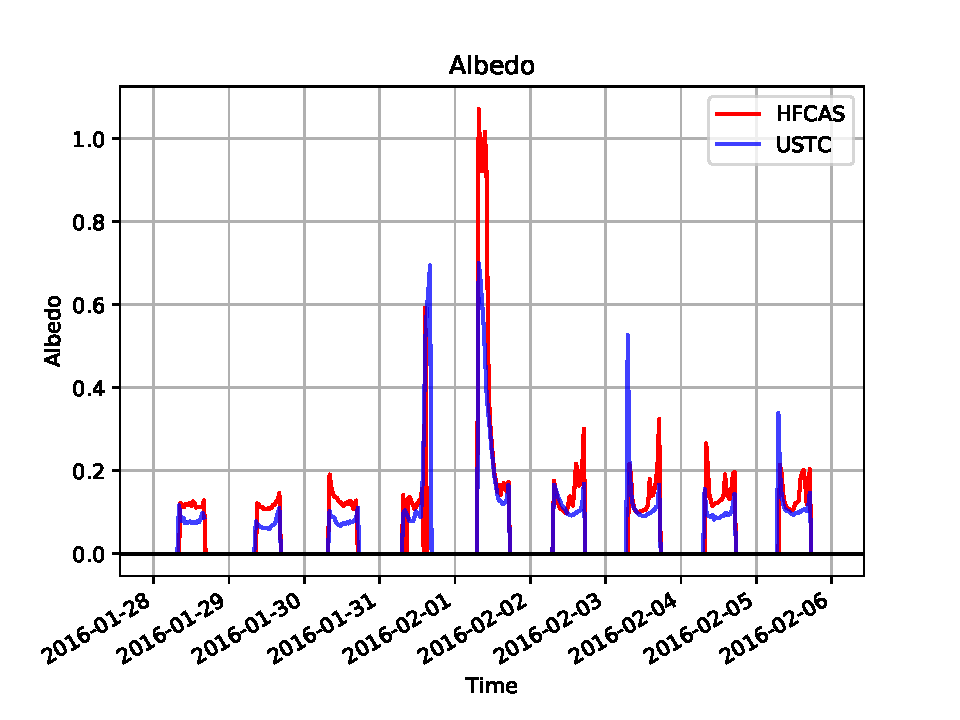
\includegraphics[width=.9\linewidth]{20160201_albedo}
\caption{2016 年 2 月 1 日附近反照率}\label{fig:20160201_albedo}
\note{图中红色表示科学岛站的反照率,蓝色表示科大站的反照率。 1 月 28 日至 1 月 31 日中午以前,反照率都比较低, 到了 1 月 31 日下午产生了一次降雪过程,反照率陡增,2 月 1 日中午逐渐衰落, 此后又维持在较低水平。 同时还可以看出与科学岛站相比,科大站的反照率要更低一些,这可能与测站地面的材质有关, 科学岛站塔下为草坪,而科大站在楼顶,下方铺有黑色防水油毡纸, 对太阳光的吸收能力更强,反射率更低。}
\end{figure}
这样便可以解释 2 月 1 日的向上短波辐射通量密度突增现象:
2 月 1 日以前持续阴天,总辐射比较低,向上反射的短波辐射也较低,
1 月 31 日产生了一次降雪,积雪使地面反照率升高,2 月 1 日天气晴朗,总辐射升高,
升高的总辐射与升高的反照率使得 2 月 1 日向上短波辐射通量密度突增,
2 月 2 日以后,积雪融化,地面反照率回复到原来较低水平,使得向上短波辐射降低。
类似地,2016 年 1 月 23 日的向上短波辐射通量密度突增也是由于地面积雪导致。
在处理向上短波辐射通量密度数据时,不应简单将这种数据当作野点。
